\label{background}
\mknote{Working on the background and looking at the related work on parallel analysis of MD traj. This section will be changing.....New work will be added soon}
\mknote{I have another idea. We can compare the performance of cpptraj with our approach for two cases of large and small tcomp/tIO. Especially we can see if cpptraj can be scaled when tcomp/tIo is small (i.e. I/O bound jobs)}

Long Tail phenomena, whereby a small proportion of task stragglers significantly impede job completion time is a big challenge toward achieving improved performance \cite{Garraghan2016}.

Over the past few years a significant amount of research has been done trying to detect and mitigate stragglers \cite{Rose2012, Dean2004, Chen2014, Bhandare2016, Kwon2012}. 
There are also works to find the stragglers root-cause in many big data processing systems \cite{Ballani2011, Ananthanarayanan2014, Jeyakumar2013, Li2014, Zaharia2012}.
Straggler root-cause has both internal and external factors. Internal factors include heterogeneous capacity of worker nodes, and resource competition due to other tasks running on the same worker node. 
External factors include resource competition due to co-hosted applications, input data skew, remote input or output source being too slow and faulty hardware \cite{Chen2014}.

Spark introduces stragglers for a number of different reasons:  1) garbage collections~\cite{Kyong2017,Ousterhout2017}, 2) JVM positioning to cores~\cite{Kyong2017}, 
2) the delay's introduced while the task moves from the scheduler to executing~\cite{Gittens2016}, 3) Disk IO during shuffling, 4) Java's just-in-time compilation~\cite{Ousterhout2017}, 
and 5) output skew \cite{Ousterhout2017}. 
In addition to these reasons, stragglers on Spark have been attributed to the overall performance of the worker or competition between resources \cite{Yang2016}.

Tuning resource allocation and tuning parallelism are other methods to improve Spark job performance. 
Many frameworks provide knobs to tune the number of parts into which an input is splitted \cite{Rose2012}. 
However, manual tuning are laborious and imprecise. 
In general, finer-grained splitting produces fewer stragglers; however, at some point the overhead of a large number of splits starts to dominate. 
Moreover, the carefully chosen value can quickly become obsolete with changes to the dataset, the processing algorithm, the runtime environment, or even when switching to a new version of the framework.

Some frameworks will identify the straggler nodes using a slow Node-Threshold. 
They identify straggler node when its performance score is less than the average performance score of all nodes and therefore prevent to launch any tasks on these slow nodes. 
The straggler node can be due to the faulty hardware or misconfiguration \cite{Dean2004}. 
However, this solution only addresses hardware-based stragglers \cite{Chen2014}.

For most of the factors causing stragglers, speculative execution and its improved versions are an effective way to solve the straggler problem. 
This technique also addresses only slow workers, but not input data skew (data imbalance) \cite{Chen2014}.

Speculative execution is a replication-based reactive straggler mitigation technique that spawns redundant copies of the slow running tasks, hoping a copy will reach completion before the original. 
This is the most prominently used in production clusters at Facebook and Microsoft Bing. 
However, without any additional information, such reactive techniques can not differentiate between nodes that are inherently slow and nodes that are temporarily overloaded \cite{Bhandare2016}.

Sampling or similar techniques can help estimate the data distribution to split the data more evenly. 
However, such statistics are often expensive to collect, insufficiently precise, or obsolete. 
Moreover, stragglers can happen even if the data distribution is balanced, due to unbalanced processing complexity for different parts of the data.

SkewTune is another technique for addressing data imbalance. 
SkewTune identifies the task with the greatest expected remaining processing time when a node becomes idle. 
The unprocessed input data of this straggling task is then pro-actively repartitioned in a way that fully utilizes the nodes in the cluster and preserves 
the ordering of the input data so that the original output can be reconstructed by concatenation \cite{Kwon2012}. 
SkewTune can significantly reduce job runtime and adds little to no overhead in the absence of skew; however, the cost of fully reading the rest of a straggler's input can be prohibitive, in particular, making 
the technique meaningless if the straggler was already dominated by the cost of reading the input.

Garraghan et al. \cite{Garraghan2016} studied stragglers on Virtualized Cloud Data-centers. 
Through statistical analysis they found that the most frequent reasons were high CPU utilization, disk utilization, unhandled IO access requests and network package loss. 
About $3\%$ to $6.5\%$ of the tasks were stragglers resulting to a $37.8\%$ to almost $50\%$ of jobs negatively impacted. 
In this study, task stragglers are defined as tasks whose execution is $150\%$ the median duration of all tasks within the same job and median task duration is used instead of mean task duration. 
This is especially because median job execution duration is less affected by extreme execution times caused by stragglers. 

The analysis performed on the trace data from Microsoft Bing's production cluster shows that $80\%$ of stragglers have a uniform probability of delay between $150-250\%$ 
compared to the median task duration, with 10\% exhibiting a delay $1000\%$ greater than median task duration \cite{Ananthanarayanan2010}.

Cloud data-flow deals with stragglers problem using dynamic work rebalancing. 
However, this method has its own technical challenges which includes data consistency, intense systematic testing, as well as a careful design, and predicting how a task will progress over time \cite{Schmidt2016}.
In addition, this approach is only effective in systems with high-throughput, low-latency task schedulers and efficient data materialization \cite{Rose2012}.

Blocked time analysis is used to measure how long each task spends blocked on a given resource. 
These approach provides a per-task measurements and allows the understanding of  straggler root-causes by correlating slow tasks with long blocked times \cite{Ousterhout2015}. 
However, the work by \cite{Ousterhout2015} does not look at a vast range of workloads nor a wide range of cluster sizes.

This work focuses on the stragglers root-cause and we are mostly trying to find how we can improve performance by identifying the underlying reasons for stragglers.


CPPTraj~\cite{cpptraj-2013} offers three levels of parallelization. The two are through MPI and the third through OpenMP.
The MPI types of parallelization CPPTraj supports are show in Figure~\ref{fig:cpptraj_arch}. In more detail,
CCPTraj allows the parallel read between frames of the same trajectory or ensemble members of
the same trajectory. When it is used to analyze a single trajectory, all frames of the trajectory
are equally distributed over the number of MPI process that are used. Each process reads the frames
that are assigned to it, executes and writes the results of all processes to the same output file.
When ensemble mode is used, each ensemble member is assigned to an MPI process. As a consequence,
there have to be as many MPI processes as ensemble members. The user has the ability to increase 
CPPTraj's throughput by assigning more than one MPI processes per ensemble member. Each ensemble 
member is divided further the same way as a single trajectory.
\begin{figure}[ht!]
		\begin{subfigure}{.5\textwidth}
		\centering
		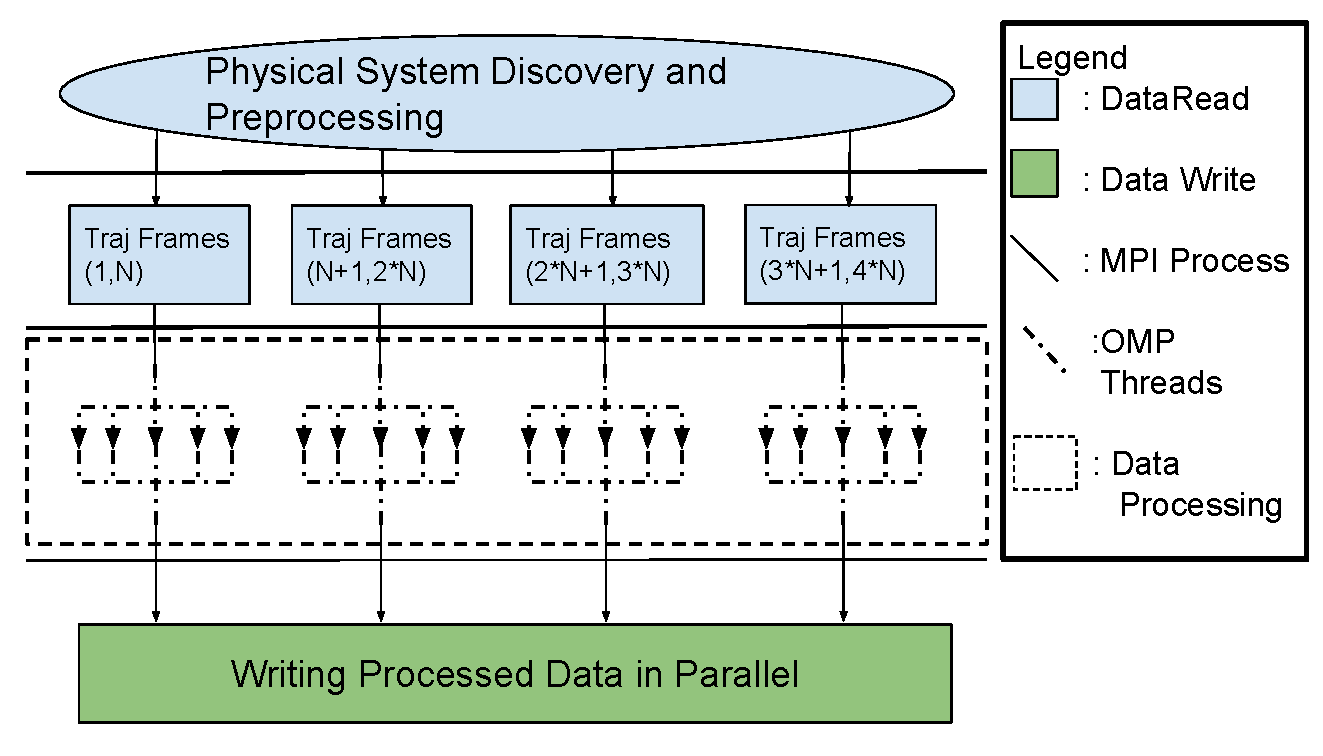
\includegraphics[width=.95\textwidth]{figures/CPPTrajExecutionSchematicSingleTrajectory.pdf}
	\end{subfigure}
	\begin{subfigure}{.5\textwidth}
		\centering
		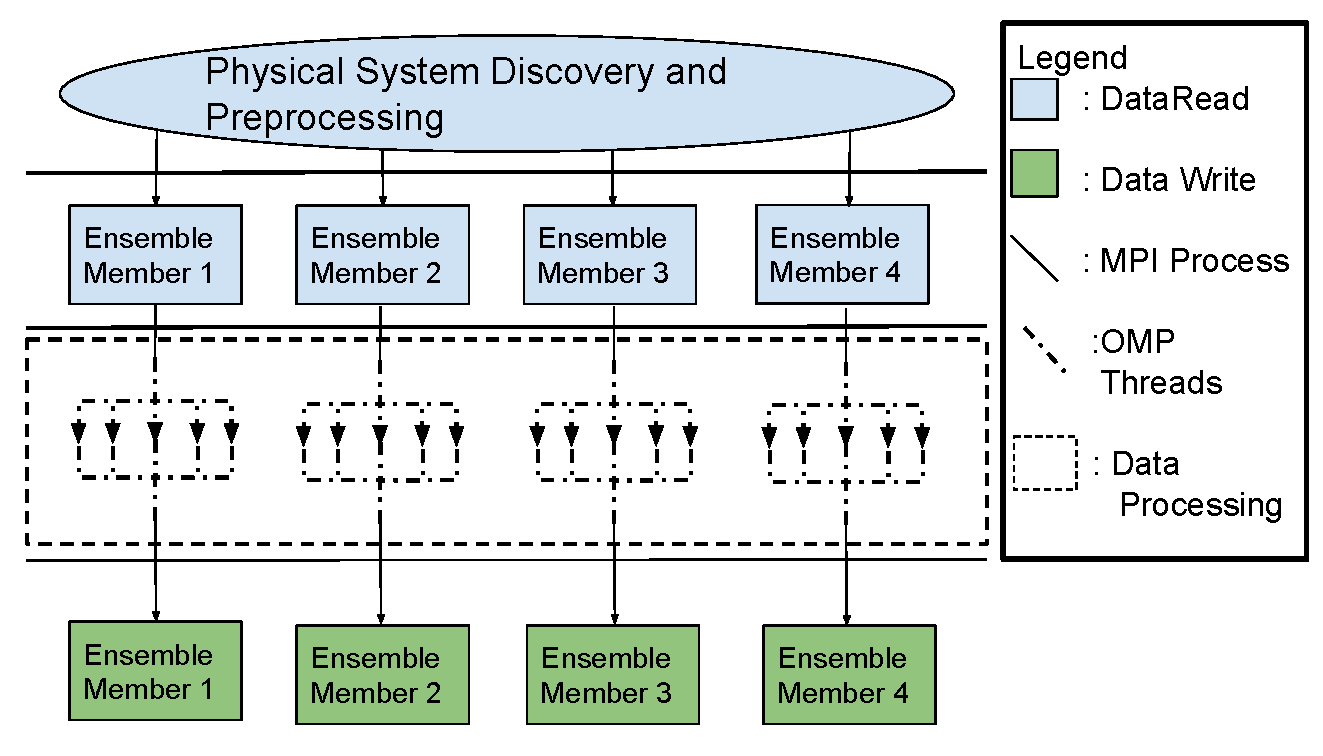
\includegraphics[width=.95\linewidth]{figures/CPPTrajExecutionSchematicEnsembleTrajectories.pdf}
	\end{subfigure}
	\caption{CPPTraj MPI modes of execution. The right figure shows the case where a single trajectory is
		given. The left figure shows the case where an ensemble of trajectories are given for analysis}
	\label{fig:cpptraj_arch}
\end{figure}

HiMach~\cite{himach-2008} was developed by D.E.Shaw Research group to provide a parallel analysis
framework for molecular dynamics simulations. HiMach extends Google's MapReduce
to provide a scalable API for MD trajectory analysis. HiMach API provides a series
of Python classes that are used to define trajectories, do per frame data acquisition
(Map class) and cross-frame analysis (Reduce class). After the user has defined all 
the above, HiMach's runtime is responsible to parallelize and distribute the Map and 
Reduce classes to the assigned cores. Data transfers between Map and Reduce phases are
done through a communication protocol created specifically for HiMach and it is transparent
from the user.